\documentclass[../../main.tex]{subfiles}

\begin{document}
\problem{4.16}
\begin{wts}
The Tietze's Extension Theorem. Let $X$ be a normal space, and for any closed subset $A\subseteq X$, and $f\in C(A,\:[a,b])$, there exists an $F\in C(X,[a,b])$ which extends $f$.
\end{wts}
\begin{proof}
We begin with an important lemma that will serve as a 'black box' for the induction.
\begin{lemma}\label{lemma:theorem-4.16}
For every $f\in C(A,\:[0,1])$, there exists a $g\in C(X, [0, 1/3])$ such that 
\begin{equation}\label{eq:1}
0\leq f-g\leq 2/3 \quad\textrm{ pointwise on } A    
\end{equation}
\end{lemma}
\begin{proof}
Since $f$ is continuous, $B=f^{-1}([0,1/3])$, and $C=f^{-1}([2/3,1])$ are closed, disjoint subsets. Applying Urysohn's Lemma (Theorem 4.15) we get a continuous function $g\in C(X,[0,1])$ such that $g|_B = 0$ and $g|_C = 1$. Rescale $g$ by a factor of $1/3$, and $g\in C(X,[0,1/3])$.\\

To show that \Cref{eq:1} holds, suppose $x\in B$, then $f(x)\in[0,1/3]$ and $g(x)=0\implies 0\leq f-g\leq 1/3\leq 2/3$. Now suppose that $x\in C$, then $f(x)\in[2/3,1]$ and $g(x)=1/3$ (recall that we relabelled $g$). So we have $0\leq 1/3\leq f-g\leq 2/3$. Lastly, for the case where $x\notin (B\cup C)$, then $f(x)\in (1/3, 2/3)$, and $g(x)\in[0, 1/3]$ implies that 
\begin{align*}
    1/3 &<    f(x) <    2/3 &\implies 1/3 \leq   f(x) \leq 2/3\\
    0   &\leq g(x) \leq 1/3 &\implies -1/3 \leq -g(x) \leq 0    
\end{align*}
Therefore $0\leq f(x)-g(x)\leq 2/3$. See \Cref{fig:theorem-4.16-error}.\\
\begin{figure}
    \centering
    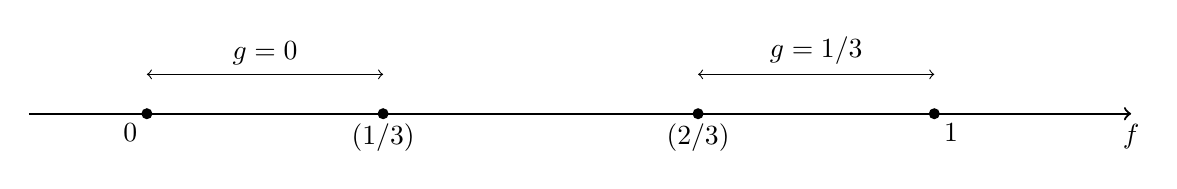
\begin{tikzpicture}
        % Draw the real line
        \draw[thick,->] (-0.5,0) -- (13.5,0) node[below] {$f$};
        
        % Left Markers
        \fill (1,0) circle (2pt);
        \fill (4,0) circle (2pt);
        \node[below left] at (1,0) {$0$};
        \node[below] at (4,0) {$(1/3)$};
        \draw[<->] (1,0.5) -- (4,0.5) node[midway,above] {$g=0$};
    
        % Right Markers
        \fill (8,0) circle (2pt);
        \fill (11,0) circle (2pt);
        \node[below right] at (11,0) {$1$};
        \node[below] at (8,0) {$(2/3)$};
        \draw[<->] (8,0.5) -- (11,0.5) node[midway,above] {$g=1/3$};
    \end{tikzpicture}
    \caption{\Cref{lemma:theorem-4.16} for Theorem 4.16: Separate the range of $f\in C(A,\:[0,1])$ into three parts. Subtract an additional $g$ that reduces the error even further.}
    \label{fig:theorem-4.16-error}
\end{figure}
\end{proof}

We can assume that $f\in C(A,\:[0,1])$, since we can relabel $f = (f-a)/(b-a)$. The main part of this proof consists of constructing a sequence of $\{g_n\}\subseteq C(X,\mathbb{R})$ where $0\leq g_n\leq (2/3)^n(1/2)$, and $0\leq f-\sum_{j\leq n}g_j\leq (2/3)^n$ on $A$. Let us begin with the base case with $n=1$. We can apply \Cref{lemma:theorem-4.16} to get $g_1\in C(X,\: [0,1/3])$
\[
0\leq f-g_1\leq (2/3)^1
\]

Now let us suppose that $\{g_j\}_{j\leq n}$ has been chosen, we will find our $g_{n+1}$ by noting that
\[
0\leq f(x)-\sum_{j\leq n}g_j(x)\leq (2/3)^n
\]
Here is where my proof deviates from that of Folland's, we multiply both sides by $(2/3)^{-n}$ and we obtain a new function in $C(A,\:[0,1])$.
\[
0\leq \left(f(x)-\sum_{j\leq n}g_j(x)\right)\left(\dfrac{3}{2}\right)^n\leq 1
\]
Applying \Cref{lemma:theorem-4.16}, we get a function $h\in C(X,[0,1/3])$ that reduces the error between $f$ and the partial sums of $g_{j\leq n-1}$. For every $x\in A$
\[
0\leq \left(f(x)-\sum_{j\leq n}g_j(x)\right)\left(\dfrac{3}{2}\right)^n-h\leq 2/3
\]
Multiplying across gives
\[
0\leq \left(f(x)-\sum_{j\leq n}g_j(x)\right)-h\left(\dfrac{2}{3}\right)^n\leq \left(\dfrac{2}{3}\right)^{n+1}
\]
Set $g_{n+1} = h\left(\dfrac{2}{3}\right)^n$ and $g_{n+1}\in C(X, [0, 2^n/3^{n+1}])$. Furthermore, the sum of all $g_j$ pointwise converges uniformly, as
\[
\sum_{j\geq 1} \norm{g_j}_u \leq \sum_{j\geq 1}\left(\dfrac{2}{3}\right)^j\cdot\dfrac{1}{2}<+\infty
\]
Denote the pointwise sum $F = \sum g_j$, then this $F\in BC(X)$ (by Theorem 4.13 and 5.1). And
\[
\bignorm{f-\sum_{j\leq n}g_j}_u\leq \left(\dfrac{2}{3}\right)^n\longrightarrow 0
\]
So $F= f$ on $A$, now if we want to obtain our $F$ on $[a,b]$ we simply relabel $F = F(b-a) + a$. This finishes the proof.
\end{proof}
\end{document}